\Chapter{A minta alkalmazás}

% TODO: Eg rövid áttekintés a könyvtári kölcsönzéses és hasonló célú alkalmazásokról. Jó, hogy ha van néhány hivatkozás is hozzá.
A mintaalkalmazás egy könyvtár internetes felületét valósítja meg. Könyvek böngészésén és kölcsönzésén kívül lehetősége van a felhasználónak könyveket értékelni, hozzászólásokat írni, listákat létrehozni, könyveket könyvjelzőkhöz adni valamint új könyvekre igényt leadni. Ebben a fejezetben az alkalmazás által nyújtott funkciók részletes bemutatásáról, valamint az alkalmazás megvalósításáról lesz szó.

\Section{Szerepkörök, használati esetek}
% TODO: Ide egy felsorolás (esetleg egy use-case diagram) kerülhet az admin és a publikus funkciókról.
Az alkalmazás use-case diagramja az alábbi ábrán található:


\bigskip

\sloppy
\noindent Egy átlagos felhasználó az alkalmazásban az alábbi funkciókat tudja igénybe venni:
\begin{itemize}
    \item Felhasználói fiókkal kapcsolatos funkciók: regisztrálás, bejelentkezés, kijelentkezés, felhasználói adatok módosítása
    \item Könyvkereséssel kapcsolatos funkciók: könyvek böngészése, könyvek szűrése, könyvek adatlapjának megnyitása
    \item Könyvekkel adatlapján igénybe vehető funkciók: könyvek értékelése, komment írása, Könyv kikölcsönözése, Könyve könyvjelzőkhöz adása, illetve eltávolítása
    \item Kölcsönzésekkel kapcsolatos funkciók: kölcsönzések böngészése, kölcsönzések meghosszabbítása, könyvek visszavitele, felhasználó kölcsönzése történetének megtekintése
    \item Könyvjelzőkkel kapcsolatos funkciók: könyvjelzők böngészése, könyvjelzők eltávolítása
    \item Listák böngészésével kapcsolatos funkciók: listák böngészése, rendezése, listák adatlapjának megtekintése, listák ajánlása
    \item Saját listákkal kapcsolatos funkciók: új lista létrehozása, lista törlése, könyv listához adása, illetve eltávolítása
    \item Könyvtárbővítéssel kapcsolatos funkciók: lehetséges könyvek közötti keresés, azok szavazásra bocsátása, szavazatra bocsátott könyvekre szavazás
\end{itemize}
\fussy

\bigskip

\noindent Admin jogosultságú felhasználó az alkalmazásban az alábbi funkciókat tudja igénybe venni:
\begin{itemize}
    \item Felhasználókkal kapcsolatos funkciók: felhasználói lista megtekintése, felhasználók kitiltása
    \item Könyvekkel kapcsolatos funkciók: új könyv könyvtárhoz adása, meglévő könyvek módosítása, illetve törlése
\end{itemize}

\begin{figure}[H]
    \centering
    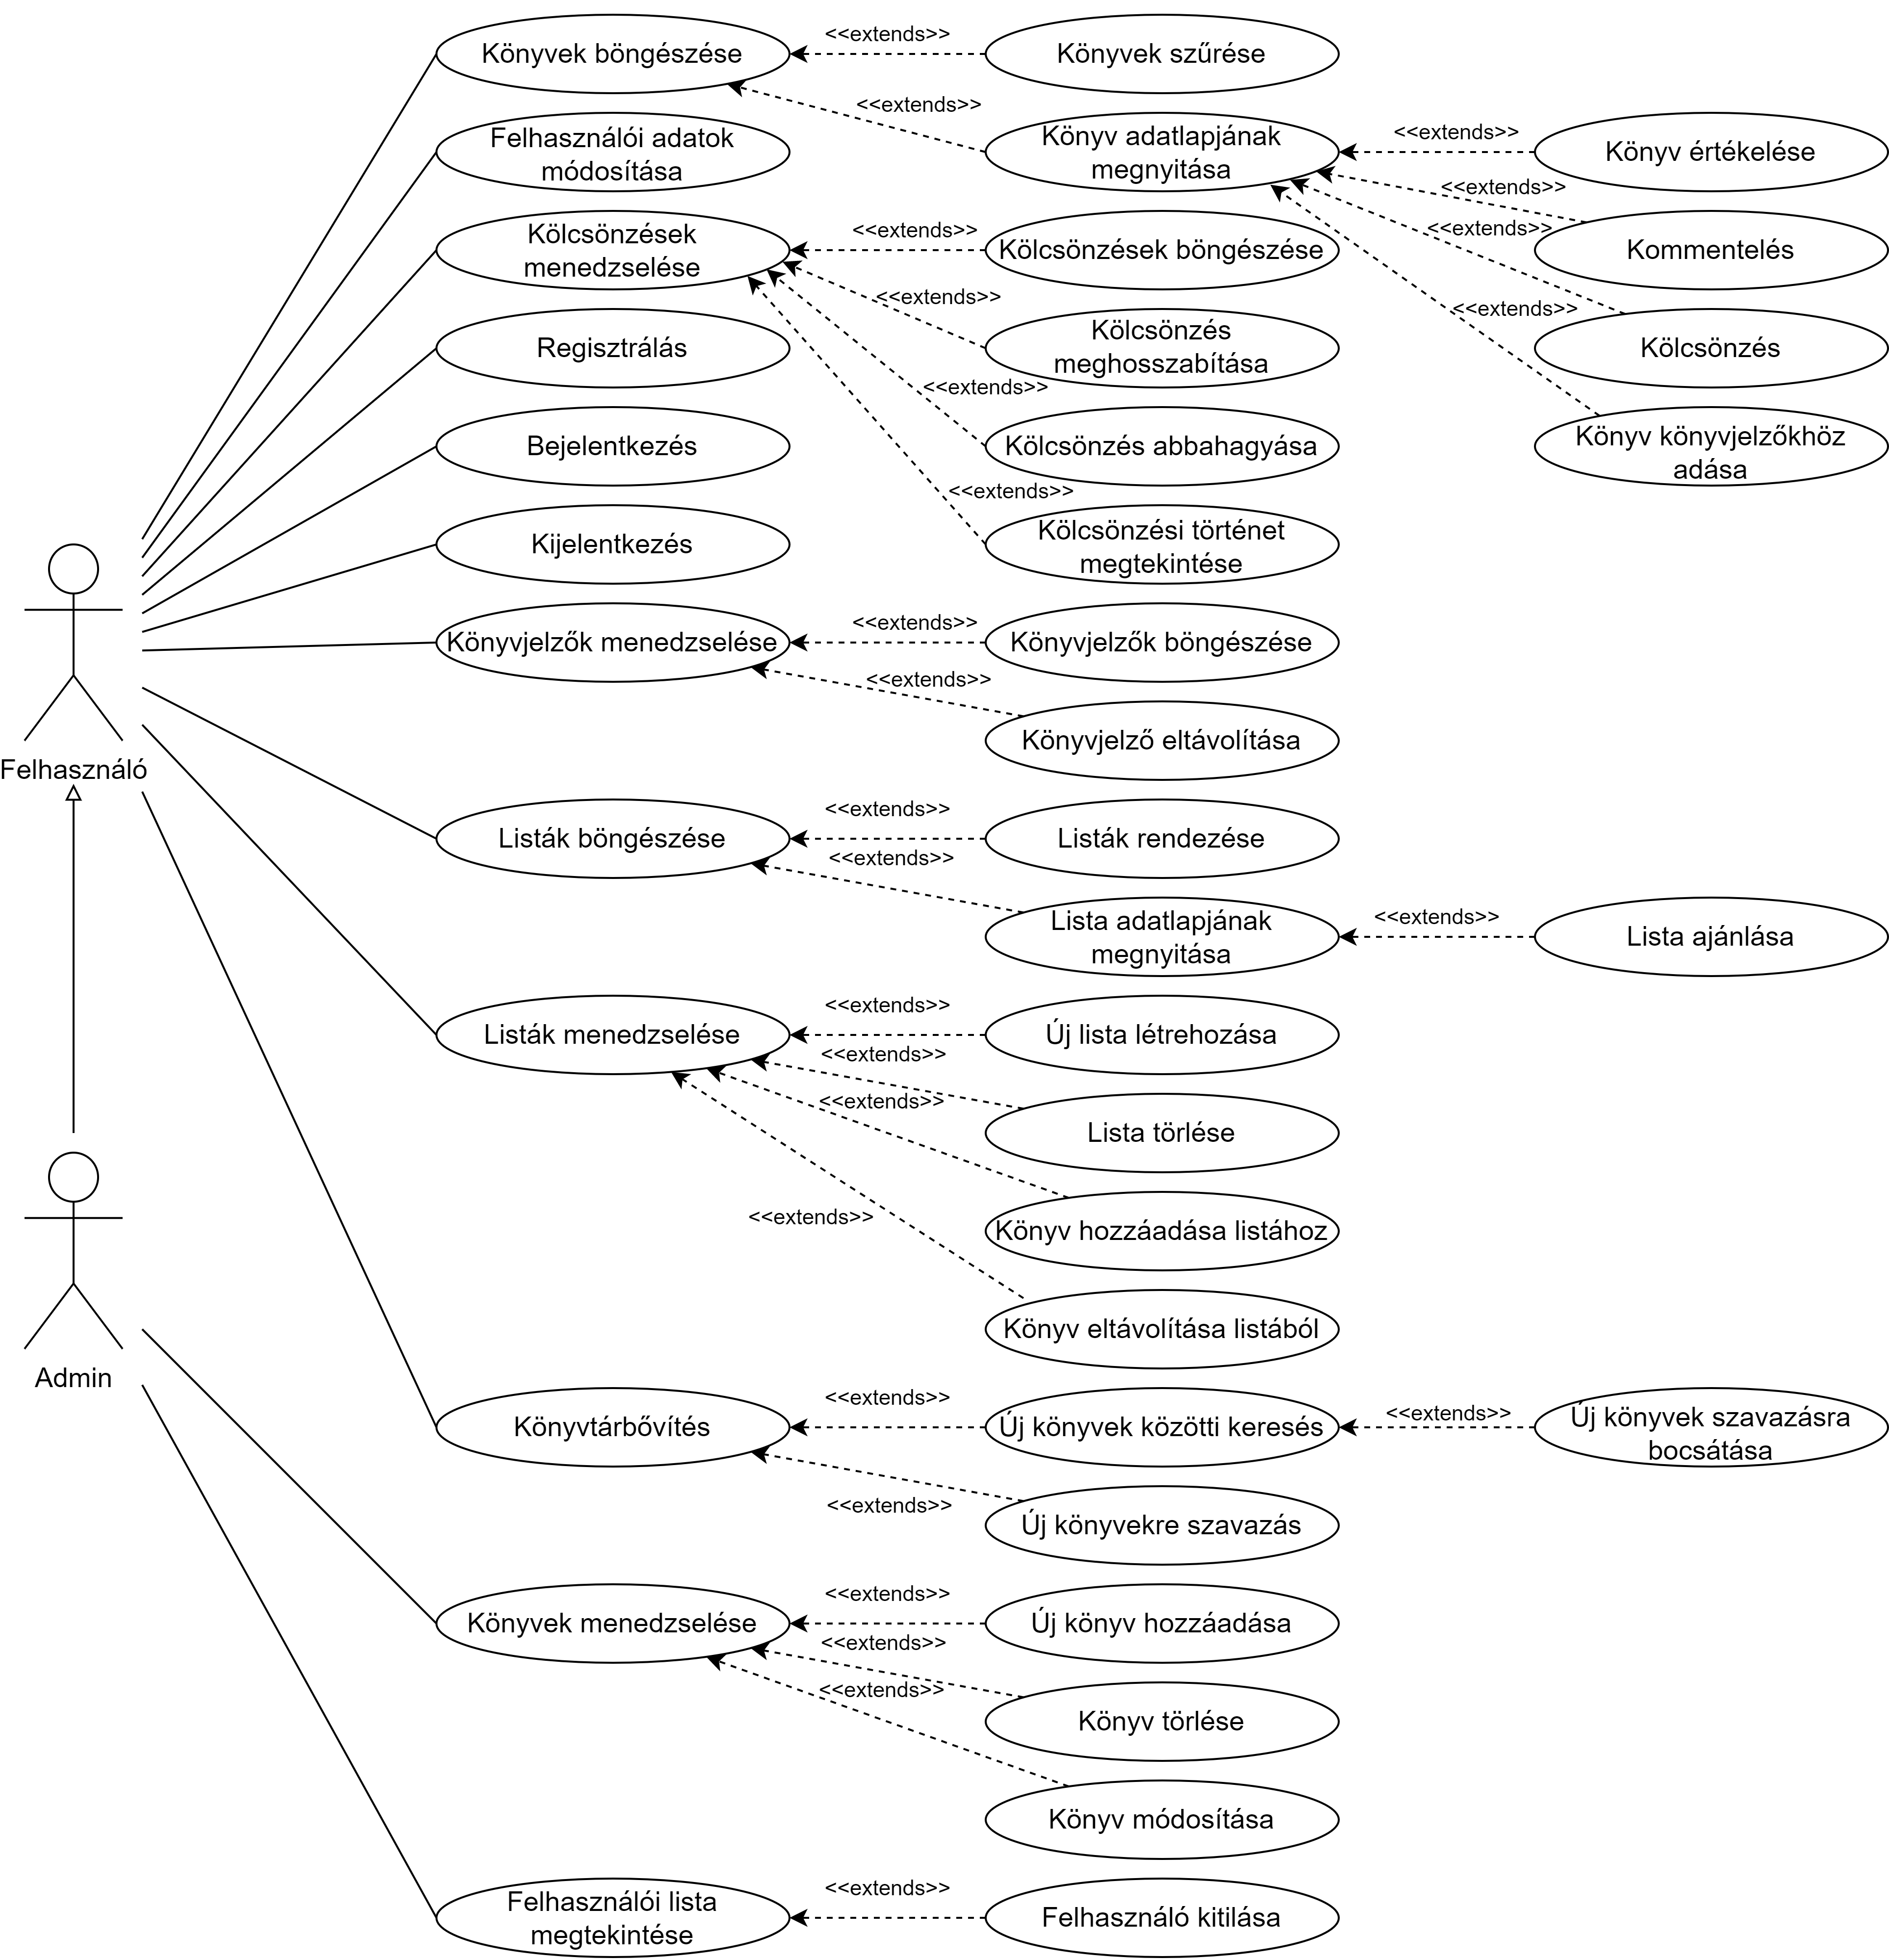
\includegraphics[scale=0.6]{images/graphlibrary-usecase-better.png}
    \caption{Az alkalmazás use-case diagramja}
\end{figure}

\Section{Funkciók, műveletek}
% TODO: Itt már részletesebben ki lehet fejteni a kölcsönzést, a listázásokat, az értékelést.
Ebben az alfejezetben bemutatásra kerül, hogy milyen funkciókkal van felruházva a mintaalkalmazás. A bemutatás az alkalmazás menüpontjain keresztül fog zajlani.

\subsection{Books menüpont}
A Books menüpont az alkalmazás központi része. Innen interaktálhat a felhasználó a könyvtárban található könyvekkel. A menüpont megnyitásakor az oldal közepén megjelennek a könyvtárban található könyvek. Egyszerre csak egy adott számú könyv jelenik meg, további könyveket a találatok alatt lévő lapszámozás funkció segítségével lehet elérni. A nyilakra kattintva egy-egy oldallal az adott irányba lehet lépni, míg egy adott számra kattintva az azzal megegyező sorszámú találatoldal fog megjelenni.

\begin{figure}[H]
\centering
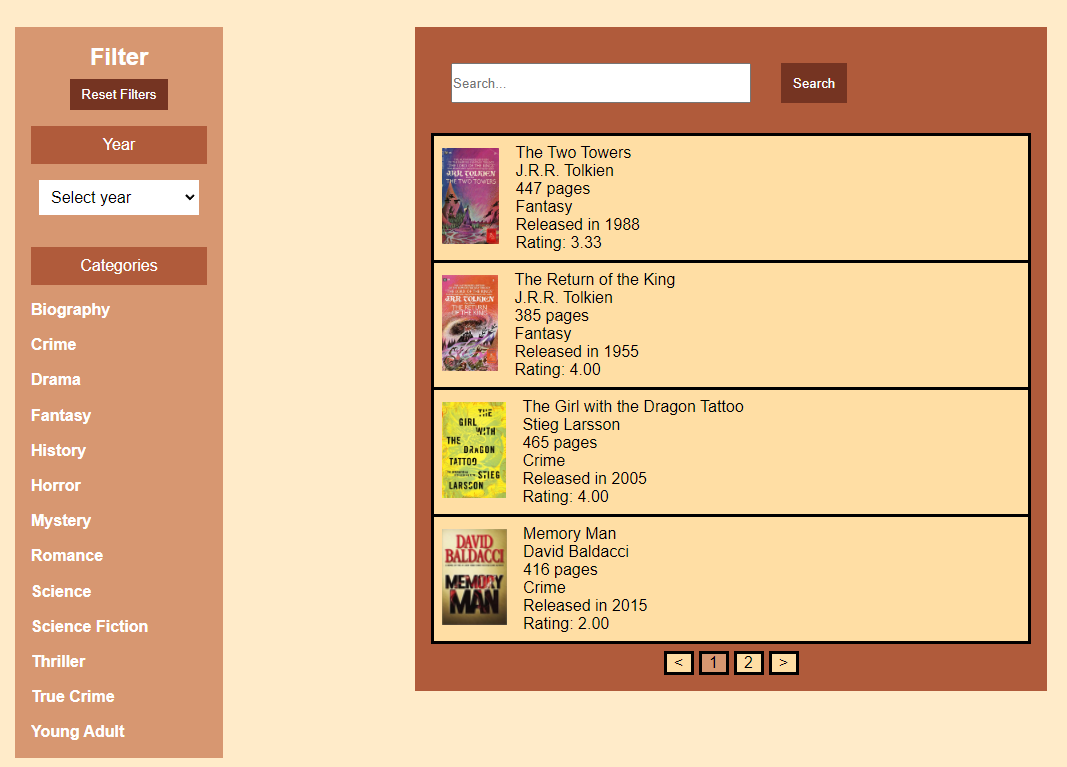
\includegraphics[scale=0.5]{images/application/books.png}
\caption{A Books menüpont}
\end{figure}

\bigskip

A megjelenő könyveket lehetősége van a felhasználónak szűrni. A könyvek felett található keresési mezőbe beírhatja a felhasználó egy könyv címét, vagy címének egy részletét, és ekkor csak keresésnek megfelelő könyvek fognak megjelenni. Ezenkívül lehetősége van még a felhasználónak a könyvektől balra található felületen megjelenési év, valamint kategória szerint is szűrni a találatokat. Ez a három szűrési lehetőség egyszerre is használható.

\bigskip

Minden megjelenő könyvhöz tartozik egy rövid összefoglaló. Ebben az összefoglalóban megtudhatja a felhasználó az adott könyv címét, a szerzőjét, hosszát, kategóriáját, megjelenési évét, borítója, valamint más a felhasználók általi értékelések átlagát. Egy összefoglalóra kattintva megjelenik az adott könyv adatlapja.



\bigskip

Egy könyv adatlapját megnyitva megjelennek a könyv adatai: 
\begin{itemize}
    \item cím
    \item szerző
    \item rövid tartalmi összefoglaló
    \item hossz
    \item kategória
    \item megjelenési év
    \item értékelések átlaga
    \item darab
\end{itemize}

\begin{figure}[H]
    \centering
    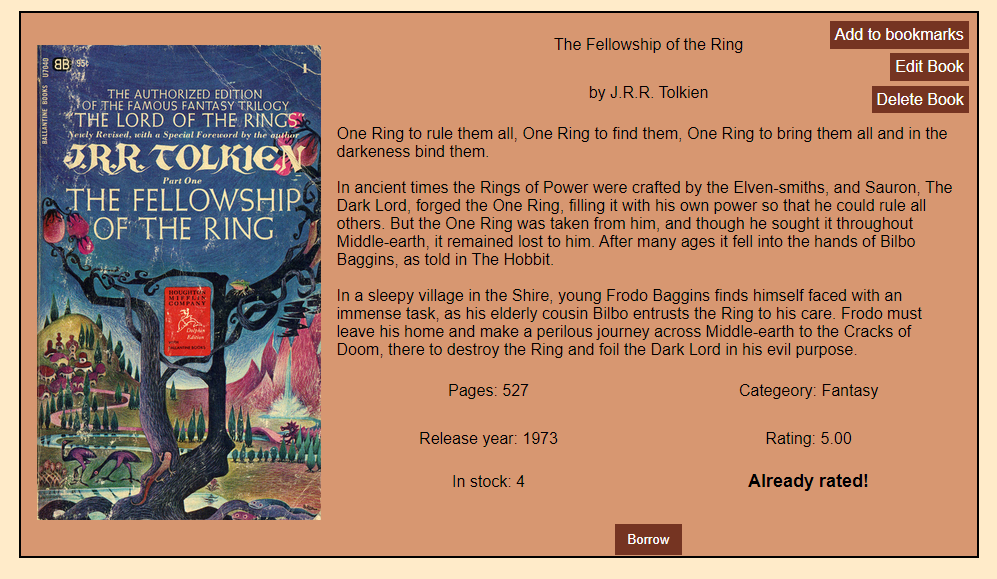
\includegraphics[scale=0.55]{images/application/bookcard.png}
    \caption{Egy könyv adatlapja}
\end{figure}

Az adatlap alatt más felhasználók által írt kommenteket találhat a felhasználó. Egy kommentnél az alábbi információk jelennek meg:
\begin{itemize}
    \item a kommentelő neve
    \item a komment írásának dátuma
    \item a komment szöveges tartalma
\end{itemize}
Egy nem bejelentkezetett felhasználónak csak az adatlap megtekintésére van lehetősége. Egy bejelentkezett felhasználó számára további funkciók is elérhetővé válnak:
\begin{itemize}
    \item Az értékelések alatt lehetősége van egy regisztrált felhasználónak a könyv értékelésére 1 és 5 között.
    \item  Az adatlap jobb felső sarkában a felhasználó a könyvjelzőihez adhatja a könyvet, vagy ha már ott volt, akkor eltávolíthatja azt onnan.
    \item  Az adatlap alján lehetősége van a felhasználónak az adott könyv kikölcsönzésére, amennyiben a könyv készleten van.
    \item  Az adatlap alatt írhat saját kommentet is a felhasználó.
\end{itemize}
 Admin jogosultsággal rendelkező felhasználónak a könyv adatlapról lehetősége van még ezeken kívül a könyvet szerkeszteni, illetve törölni.

\subsection{Lists menüpont}
A Lists menüpontban lehetősége van a felhasználónak más felhasználók által készített listák megtekintésére, valamint saját listák menedzselésére. 

\bigskip

A Browse Lists almenüpontra kattintva megjelennek a felhasználók által készített listák. A Books menüponthoz hasonlóan itt a lapszámozás funkció segítségével válthat a felhasználó a listák között. A listákat lehetősége van a felhasználónak ajánlások, illetve létrehozási dátum szerint rendezni. Minden listához tartozik egy összefoglaló, ami az alábbiakat tartalmazza:
\begin{itemize}
    \item a lista neve
    \item a listában levő könyvek száma
    \item az ajánlások száma
    \item a lista létrehozásának dátuma
\end{itemize}
 Egy lista összefoglalójára kattintva megjelenik a lista adatlapja.

\bigskip

\begin{figure}[H]
    \centering
    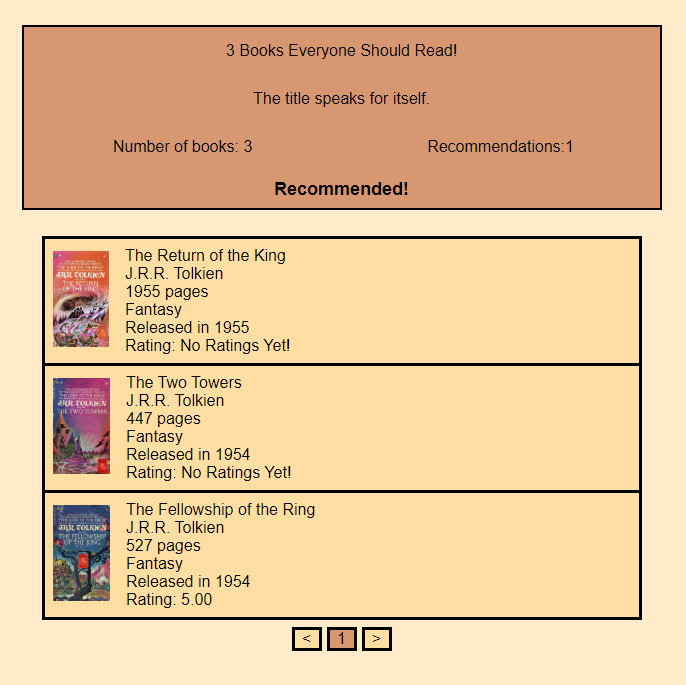
\includegraphics[scale=0.65]{images/application/listcard.png}
    \caption{Egy lista adatlapja}
\end{figure}

\noindent A lista adatlapján az alábbiak szerepelnek:
\begin{itemize}
    \item a lista neve
    \item a lista leírása
    \item listában levő könyvek száma
    \item az ajánlások száma.
\end{itemize}

Az adatlap alatt láthatja a felhasználó, hogy pontosan mely könyvek vannak a listában. Bejelentkezett felhasználónak lehetősége van a lista ajánlására.

\bigskip

A New List menüpontban a felhasználó egy listanév és egy leírás megadásával saját listát hozhat létre. A felhasználó a saját listáit a Delete List menüpontban törölheti.

\bigskip

Az Add Books To List menüpontban lehetősége van a felhasználónak kiválasztania egyet a listáit közül. Egy lista kiválasztása utána a "Books" menüpont felülete jelenik meg annyi különbséggel, hogy minden könyv elemhez tartozik egy Add gomb, amivel az adott könyv a listához rendelhető. A Remove Book From List menüpontban a lista kiválasztása után megjelennek a listához tartozó könyvek, melyeket a Remove gombra kattintva lehet eltávolítani az adott listából.

\subsection{Expand menüpont}
Az Expand menüpont lehetőséget nyújt a felhasználók számára, hogy a könyvtárban még nem található könyvekkel bővítsék a könyvtár készletét. 

\bigskip

Az Add almenüpontban lehetősége van a felhasználónak cím, író és kategória szerint keresni a Google Books katalógusában. Keresés utána megjelennek a találatok, melyekhez tartozik egy-egy rövid összefoglaló, amely az alábbiakat tartalmazza:
\begin{itemize}
    \item cím
    \item író
    \item oldalszám
    \item kategória
    \item megjelenési év
    \item tartalmi összegzés (kattintás után)
\end{itemize}
Minden találathoz tartozik egy Add gomb, amire ha rákattint a felhasználó, akkor a könyv szavazásra bocsátódik.

\bigskip

A Vote almenüpontban lehetősége van a felhasználónak szavazásra bocsátott könyvekre szavazni. Ha egy könyv elég szavazatot gyűjt, akkor az hozzáadódik a könyvtárhoz.

\begin{figure}[H]
    \centering
    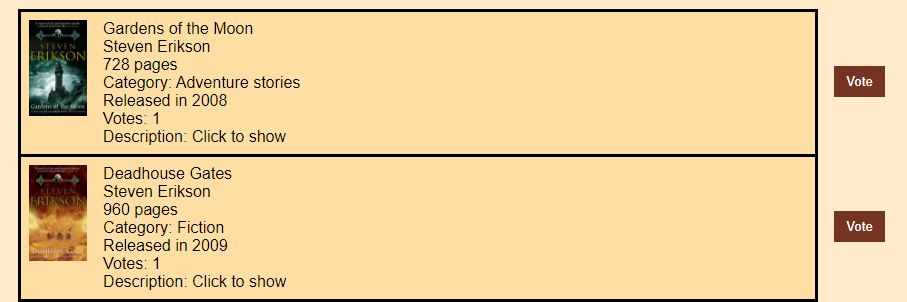
\includegraphics[scale=0.6]{images/application/expand.png}
    \caption{Bővítés menüpont - Szavazás funkció}
\end{figure}

\subsection{Borrowings menüpont}
A Borrowings menüpontban tudja a felhasználó megtekinteni a jelenlegi kölcsönzéseit. A könyvek a rövid összefoglaló formájukban jelennek meg. Minden megjelenő könyvtől jobbra találhatóak a kölcsönzéssel kapcsolatos információk, illetve lehetőségek. 

\begin{figure}[H]
    \centering
    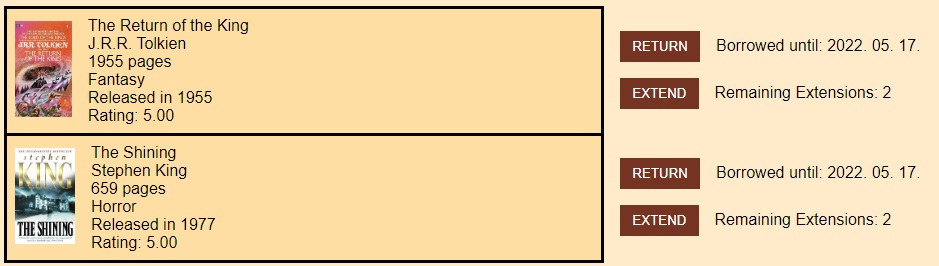
\includegraphics[scale=0.6]{images/application/borrowings.png}
    \caption{Kölcsönzések menüpont}
\end{figure}

\bigskip

Egy könyv kikölcsönzése alapvetően 30 napig tart. Ezt az időtartamot a felhasználónak kétszer van lehetősége meghosszabbítani, mindegyik hosszabbítás 30 napot ad a teljes időtartamhoz, tehát egy felhasználó egy könyvet maximum 90 napig birtokolhat. Azt, hogy hány hosszabbítási lehetősége van a felhasználónak, és hogy meddig tart a kölcsönzési határidő, a könyvtől jobbra található részen láthatja a felhasználó. Az Extend gombra kattintva megtörténik a hosszabbítás, a Return gombra kattintva pedig a felhasználó visszaadja a könyvet a könyvtárnak. 

\subsection{Bookmarks menüpont}
A Bookmarks menüpontban megtekintheti a felhasználó a könyvjelzőit. A könyvek a rövid összefoglaló formájukban jelennek meg. Minden könyvhöz tartozik egy Remove gomb, amivel a felhasználó eltávolíthatja a könyvet a könyvjelzők közül.

\begin{figure}[H]
    \centering
    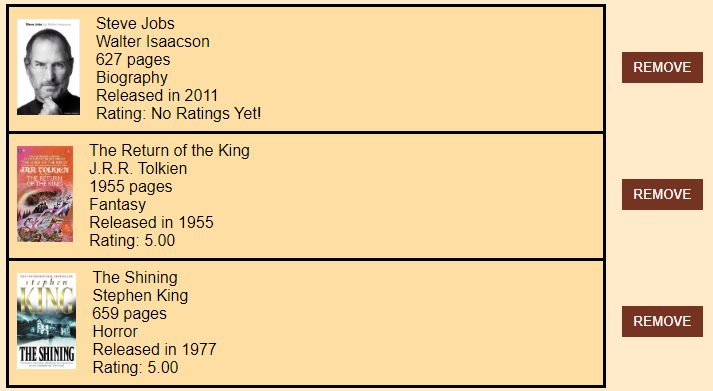
\includegraphics[scale=0.65]{images/application/bookmarks.png}
    \caption{Könyvjelzők menüpont}
\end{figure}

\subsection{Signup menüpont}
A Signup menüpontban hozhat létre a felhasználó saját felhasználói fiókot. Egy ilyen felhasználói fiók szükséges ahhoz, hogy az alkalmazás legtöbb funkciója igénybe vehető legyen. A regisztrációhoz meg kell adni egy nevet, egy egyedi email címet és egy jelszót. Már foglalt email cím megadási esetén a felhasználó hibaüzenetet kap.

\subsection{Login menüpont}
A Login menüpontban léphet be a felhasználó a létrehozott felhasználói fiókjába helyes email cím és jelszó kombináció megadása után. Hibás kombináció megadása esetén a felhasználói hibaüzenetet kap.

\subsection{Profile menüpont}
A History gombra kattintva megtekintheti a felhasználó, hogy milyen korábbi kölcsönzései voltak.

\bigskip

A Change User Data gombra kattintva lehetősége van a felhasználónak a nevét, jelszavát és/vagy email címét megváltoztatni a jelenlegi jelszó megadása után. Hibás jelszó megadása esetén a felhasználó hibaüzenetet kap.

\subsection{Admin menüpont}
Az Admin menüponthoz csak az admin jogosultsággal rendelkező felhasználóknak van hozzáférési joga. 

\bigskip

Az Add New Book gombra kattintva megjelenik egy űrlap, amelyen meg tudja adni az admin az új könyv címét, szerzőjét, rövid tartalmi összegzését, hosszát, kategóriáját, megjelenési évét, borítóját, és hogy hány darab van a könyvből készleten. Az Add Book gombra kattintva az űrlapon megadott könyv hozzáadódik a könyvtárhoz. 

\begin{figure}[H]
    \centering
    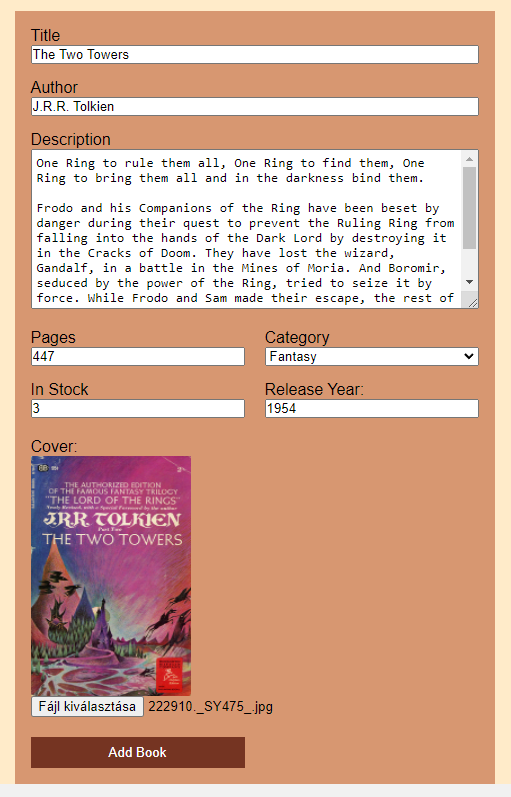
\includegraphics[scale=0.7]{images/application/newbook.png}
    \caption{Új könyv hozzáadása}
\end{figure}

A User List gombra kattintva megjelenik az összes felhasználó neve és email címe. A Ban user gombra kattintva lehetősége van az adminnak egy felhasználó végleges kitiltására.

\begin{figure}[H]
    \centering
    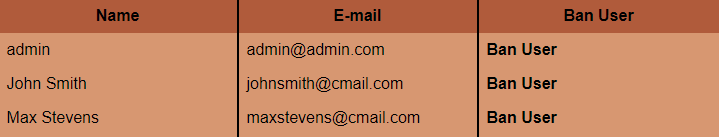
\includegraphics[scale=0.7]{images/application/userlist.png}
    \caption{Felhasználói lista}
\end{figure}

\Section{Az alkalmazás architektúrája}
% TODO: Ide kellene egy áttekintő jellegű ábra az "elkészítendő" alkalmazás szerkezetéről. Ez mutatná be, hogy a felhasznált technológiák hogyan kapcsolódnak egymáshoz.

Az alkalmazás architektúráját az alábbi ábra ábrázolja:

\begin{center}
   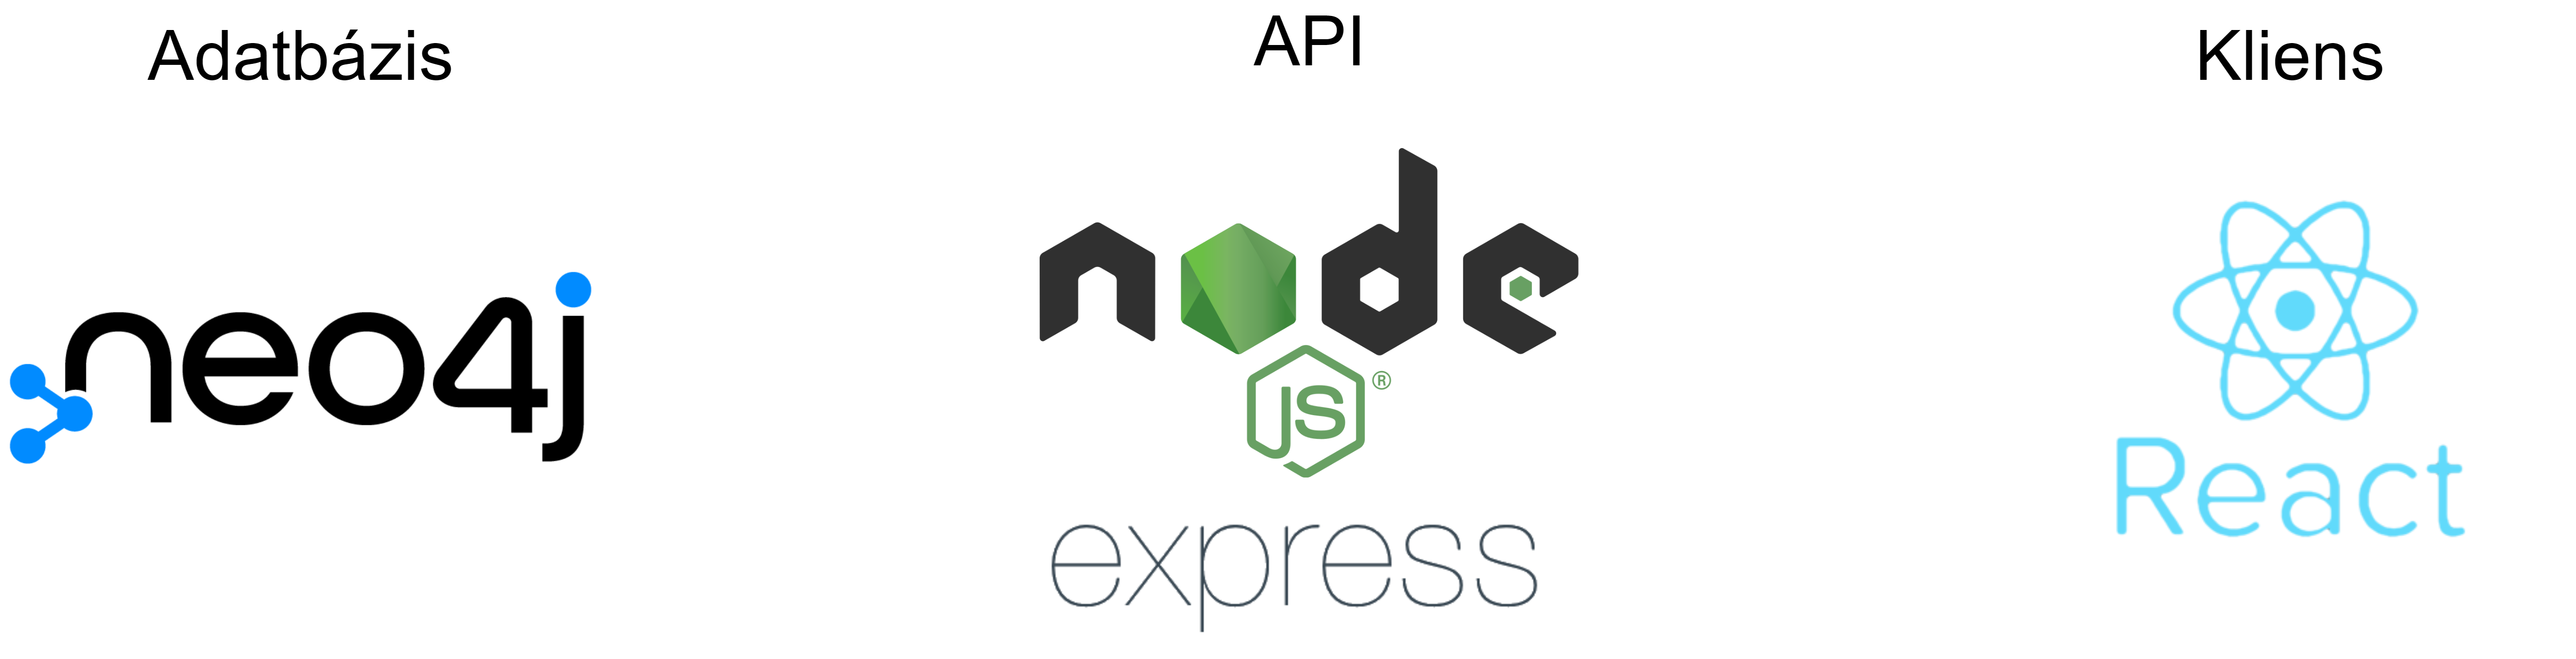
\includegraphics[scale=0.3]{images/graphlibrary_architecture.png}
\end{center}

A kliens a React könyvtár segítségével valósul meg. Az adatok a Neo4j gráfadatbázisban kerülnek tárolásra. A kettő közötti kommunikációt a NodeJS és az Express keretrendszer teszi lehetővé.

\Section{Az API}
Ebben az alfejezetben található az API tömör leírása. Az API részletes OpenAPI szabvány szerinti leírása külön fájlban megtalálható.

\subsection{Könyvekkel kapcsolatos operációk}
\renewcommand\tabularxcolumn[1]{m{#1}}
\begin{center}
\begin{table}[H]
\begin{tabularx}{\textwidth}{ |l|c|Y|Y| } 
 \hline
 \multicolumn{1}{|c|}{\textbf{Útvonal}} & \textbf{Metódus} & \textbf{Paraméterek} & \textbf{Feladat} \\ 
 \hhline{|=|=|=|=|}
 /book & POST & Könyv objektum & Új könyv létrehozása  \\ 
 \hline
 /book & GET & Keresési feltételek, Pagination adatok & Könyvek visszaadása  \\ 
 \hline
 /book & DELETE & Könyv ID & Könyv törlése  \\ 
 \hline
 /book & PUT & Könyv objektum & Könyv módosítása  \\ 
 \hline
 /book/list/\{listOfIds\} & GET & Könyv ID-k listája, Pagination adatok & Könyvek visszaadása  \\ 
 \hline
 /book/\{bookId\} & GET & Könyv ID & ID-nek megfelelő könyv visszaadása  \\ 
 \hline
 /book/rate & POST & Könyv és Felhasználó ID, Értékelés & Új értékelés hozzáadása  \\ 
 \hline
\end{tabularx}
\caption{Book operációk}
\end{table}
\end{center}

\subsection{Kommentekkel kapcsolatos operációk}
\begin{center}
\begin{table}[H]
\begin{tabularx}{\textwidth}{ |l|c|Y|Y| } 
 \hline
 \multicolumn{1}{|c|}{\textbf{Útvonal}} & \textbf{Metódus} & \textbf{Paraméterek} & \textbf{Feladat} \\ 
 \hhline{|=|=|=|=|}
 /comment/\{bookId\} & GET & Könyv ID & Könyvhöz tartozó kommentek visszaadása  \\ 
 \hline
 /comment & POST & Komment objektum & Új komment létrehozása  \\ 
 \hline
\end{tabularx}
\caption{Comment operációk}
\end{table}
\end{center}

\subsection{Listákkal kapcsolatos operációk}
\begin{center}
\begin{table}[H]
\begin{tabularx}{\textwidth}{ |l|c|Y|Y| } 
 \hline
 \multicolumn{1}{|c|}{\textbf{Útvonal}} & \textbf{Metódus} & \textbf{Paraméterek} & \textbf{Feladat} \\ 
 \hhline{|=|=|=|=|}
 /list & POST & Lista objektum & Új lista létrehozása  \\ 
 \hline
 /list & GET & Pagination információk, Rendezési sorrend & Lista visszaadása  \\ 
 \hline
 /list & DELETE & Lista ID & Lista törlése  \\ 
 \hline
 /list/user\{userId\} & GET & Felhasználó ID & Felhasználó listáinak visszaadása  \\ 
 \hline
 /list/\{listId\} & GET & Könyv objektum & ID-nek megfelelő lista visszaadása  \\ 
 \hline
 /list/book & POST & Könyv ID, Lista ID & Könyv listához adása  \\ 
 \hline
 /list/book & DELETE & Könyv ID, Lista & Könyv törlése listából  \\ 
 \hline
 /list/recommendation & POST & Lista ID & Új ajánlás hozzáadása  \\ 
 \hline
\end{tabularx}
\caption{List operációk}
\end{table}
\end{center}

\subsection{Bővítéssel kapcsolatos operációk}
\begin{center}
\begin{table}[H]
\begin{tabularx}{\textwidth}{ |l|c|Y|Y| } 
 \hline
 \multicolumn{1}{|c|}{\textbf{Útvonal}} & \textbf{Metódus} & \textbf{Paraméterek} & \textbf{Feladat} \\ 
 \hhline{|=|=|=|=|}
 /expand & POST & Könyv objektum, Felhasználó ID & Új potenciális könyv létrehozása  \\ 
 \hline
 /expand & GET & Pagination információk & Potenciális könyvek visszaadása  \\ 
 \hline
 /expand & DELETE & Könyv ID & Potenciális könyv eltávolítása  \\ 
 \hline
 /expand/vote & POST & Könyv ID, Felhasználó ID & Új szavazás hozzáadása  \\ 
 \hline
\end{tabularx}
\caption{Expand operációk}
\end{table}
\end{center}

\subsection{Kölcsönzésekkel kapcsolatos operációk}
\begin{center}
\begin{table}[H]
\begin{tabularx}{\textwidth}{ |l|c|Y|Y| } 
 \hline
 \multicolumn{1}{|c|}{\textbf{Útvonal}} & \textbf{Metódus} & \textbf{Paraméterek} & \textbf{Feladat} \\ 
 \hhline{|=|=|=|=|}
 /borrow/\{userId\} & GET & Felhasználó ID & Felhasználó kölcsönzéseinek visszaadása\\ 
 \hline
 /borrow & POST & Kölcsönzés objektum & Új Kölcsönzés létrehozása  \\ 
 \hline
 /borrow & DELETE & Kölcsönzés objektum & Kölcsönzés törlése \\ 
 \hline
 /borrow/extend & POST & Kölcsönzés objektum & Kölcsönzés meghosszabbítása \\ 
 \hline
\end{tabularx}
\caption{Borrow operációk}
\end{table}
\end{center}

\subsection{Könyvjelzőkkel kapcsolatos operációk}
\begin{center}
\begin{table}[H]
\begin{tabularx}{\textwidth}{ |l|c|Y|Y| } 
 \hline
 \multicolumn{1}{|c|}{\textbf{Útvonal}} & \textbf{Metódus} & \textbf{Paraméterek} & \textbf{Feladat} \\ 
 \hhline{|=|=|=|=|}
 /bookmarks/\{userId\} & GET & Felhasználó ID & Felhasználó könyvjelzőinek visszaadása\\ 
 \hline
 /bookmarks & POST & Könyvjelző objektum & Új könyvjelző létrehozása  \\ 
 \hline
 /bookmarks & DELETE & Könyv objektum & Könyvjelző törlése \\ 
 \hline
\end{tabularx}
\caption{Bookmarks operációk}
\end{table}
\end{center}

\subsection{Felhasználókkal kapcsolatos operációk}
\begin{center}
\begin{table}[H]
\begin{tabularx}{\textwidth}{ |l|c|Y|Y| } 
 \hline
 \multicolumn{1}{|c|}{\textbf{Útvonal}} & \textbf{Metódus} & \textbf{Paraméterek} & \textbf{Feladat} \\ 
 \hhline{|=|=|=|=|}
 /user & POST & Felhasználó objektum & Új felhasználói fiók létrehozása  \\ 
 \hline
 /user & GET & - & Felhasználók visszaadása  \\ 
 \hline
 /user & PUT & Felhasználó objektum & Felhasználó módosítása  \\ 
 \hline
 /user & DELETE & Felhasználó ID & Felhasználói fiók törlése  \\ 
 \hline
 /user/login & POST & Bejelentkezési adatok & Felhasználói fiókba való bejelentkezés \\ 
 \hline
\end{tabularx}
\caption{User operációk}
\end{table}
\end{center}

\subsection{Kölcsönzési történettel kapcsolatos operációk}
\begin{center}
\begin{table}[H]
\begin{tabularx}{\textwidth}{ |l|c|Y|Y| } 
 \hline
 \multicolumn{1}{|c|}{\textbf{Útvonal}} & \textbf{Metódus} & \textbf{Paraméterek} & \textbf{Feladat} \\ 
 \hhline{|=|=|=|=|}
 /historyborrow & POST & Felhasználó ID, Könyv ID, Dátum & Kölcsönzés naplózása  \\ 
 \hline
 /historyborrow/\{userID\} & GET & Felhasználó ID, Pagination információk & Kölcsönzése történet visszaadása  \\ 
 \hline
\end{tabularx}
\caption{Historyborrow operációk}
\end{table}
\end{center}

\Section{A kliens alkalmazás}
% TODO: Be kellene mutatni, hogy a kliens milyen nagyobb részekből épül fel. Az implementáció
%Általános React információk, alapvető kliens felépítés, információk

% https://hu.reactjs.org/tutorial/tutorial.html#what-is-react idézet:
A kliens alkalmazás a React könyvtárral valósul meg. "A React egy deklaratív, effektív, és rugalmas JavaScript könyvtár, felhasználói felületek készítéséhez. Lehetővé teszi komplex felhasználói felületek összeállítását izolált kódrészletekből, amiket “komponenseknek” hívunk." \cite{react}

A komponensek közötti adatcsere úgynevezett propokkal vannak megvalósítva. Például:
\begin{lstlisting}
    <BookItem
        title={"The Fellowship of the Ring"}
        author={"J.R.R. Tolkien"}
     />
\end{lstlisting}
Ebben a példában a BookItem komponens két propot kap, title és book, amiket a komponens később fel tud használni. Ahhoz, hogy ezek elérhetők legyenek, a komponens deklarációjakor be kell állítani, hogy fogadjon propokat:
\begin{lstlisting}
    const BookItem = (props) => {...}
\end{lstlisting}

Ezután például a title prop értékét meg lehet kapni a props.title-re utalva.

\bigskip

Az alkalmazás inicializálása a create-react-app eszközzel történik, aminek a lépései a következők Node package manager esetében:
\begin{itemize}
    \item npm install -g create-react-app parancs futtatása, ami telepíti az eszközt
    \item npm init react-app my-app parancs futtatása, ami inicializálja a React alkalmazást
    \item npm start parancs futtatása, ami elindítja az alkalmazást
\end{itemize}

\bigskip
A useState React Hook segítségével deklarálhatunk úgynevezett állapot változókat. Ezek olyan változók, amelyek a komponens újrarenderelésekor nem veszítik el értéküket. Például:
\begin{lstlisting}
  const [book, setBook]=useState("The Fellowship of the Ring")
\end{lstlisting}
Itt a book a változó, aminek kezdőértéke a The Fellowship of the Ring string. A változó értékét a setBook függvénnyel lehet megváltoztatni:
\begin{lstlisting}
  setBook("The Two Towers")
\end{lstlisting}
Ezzel a változó értéke a "The Two Towers" stringre változik. A változó értékének változásakor a komponens újrarenderelődik.

%useeffect, cleanup
\begin{lstlisting}
  useEffect(() => {
    getBook(bookId).then((data) => {
      setBook(data);
    });
  }, [bookId]);
\end{lstlisting}

Ebben a useEffect-ben található kód lefut, hogy ha a bookId értéke megváltozik. Futáskor küld egy GET request-et a backendnek, majd a megkapott adatot átadja a book állapot változónak a setBook függvényt felhasználva. Viszont, ha a kérés elküldése, és a setBook függvény futása között a komponens úgymond lecsatlakozik, tehát például átlépünk egy olyan részére az alkalmazásnak, ahol az adott komponens nincs renderelve, akkor memory leak-et kapunk. Ennek elkerülése érdekében egy cleanup függvényt kell tennünk a useEffect-be. A cleanup függvény lefut a komponens lecsatlakozásakor. A cleanup függvény alakja:

\begin{lstlisting}
    return () => {...}
\end{lstlisting}
Tehát a kiegészített useEffect Hook így fog kinézni:
\begin{lstlisting}
  useEffect(() => {
    let isActive = true;
    getBook(bookId).then((data) => {
      if (isActive) {
        setBook(data);
      }
    });

    return () => {
      isActive = false;
    };
  }, [bookId]);
\end{lstlisting}
Ebben az esetben, a setBook csak akkor fut le, hogy ha az isActive változó igaz. A komponens lecsatlakozásakor le fog futni a cleanup függvény, tehát az isActive értéke hamis lesz, tehát a setBook nem fog lefutni, így nem lesz memory leak.

\bigskip

A továbbiakban az alkalmazás komponensei kerülnek bemutatásra.

\subsection{Navigáció}
Az oldalon történő navigáció a React Router segítségével van megvalósítva. A React Rotuer egy React könyvtár, aminek fő célja, hogy segítse a komponensek közötti navigációt. Ehhez először az index.js fájlban az App komponenst BrowserRouter komponensbe kell helyezni:  
\begin{lstlisting}
     <BrowserRouter>
      <App />
    </BrowserRouter>     
\end{lstlisting}

Ezután az App.js fájlban a Switch komponensbe lehet írni a különböző Route-okat. A Switch komponens az első egyező útvonalú Route-ot fogja renderelni. A Route szintén egy komponens, amelynek a path paraméterében lehet megadni a kívánt elérési útvonalat, majd a komponensbe el lehet helyezni a renderelni kívánt komponenst, például: 
\begin{lstlisting}
    <Route path="/books" exact>
      <BooksPage />
    </Route>    
\end{lstlisting}

Ez azt jelenti, hogy ha az útvonal pontosan /books (az exact miatt), akkor a BooksPage komponens lesz renderelve. Egy route elérése feltételhez is szabható, például így: 
\begin{lstlisting}
    {authCtx.isLoggedIn && (
      <Route path="/profile">
        <ProfilePage />
      </Route>
    )}
\end{lstlisting}

Így csak akkor renderelődik a ProfilePage komponens, ha a felhasználó be van jelentkezve. Van lehetőség arra is, hogy ha egyik útvonalra se illik a megadott URL, akkor egy bizonyos komponens legyen renderelve. Ez úgy érhető el, hogy az utolsó Route komponensnek path="*" paramétert adunk.

\subsection{Authentication Context}
%bővíthető
A Context API segítségével egyszerűsíteni lehet a komponensek közötti adatcserét. Ebben az alkalmazásban a felhasználóhoz tartozó információk tárolására van felhasználva a Context API. Mivel a felhasználói adatok szinte minden komponensben fel vannak használva valamilyen módon, célszerű volt ezt a megoldást implementálni. 

\bigskip

A context az auth-context.js fájlban van inicializálva. A context először bejelentkezéskor kap értéket. Bizonyos komponensekben ezek az értékek változhatnak, bővülhetnek. A komponensek a useContext React Hook-al tudják elérni a context-et.

\subsection{Books komponensek}
Az alábbi komponensek felelősek a Books menüpont megvalósításáért.

\subsubsection{BooksContent komponens}
A BooksContent felelős a Books menüpontért, valamint a Lists menüpont Add Books To List funkciójáért. Felhasználja a BookFilters és a BookList komponenseket.

\bigskip

A könyvek szűréséhez felhasználja a useHistory és useLocation React Router Hook-okat. A komponens az URL-ben található query paramétereket használja fel a szűréshez, ez lehetővé teszi, hogy a megfelelő URL-t felhasználva egy specifikus szűrést kapjunk. Például, a /books?category=Fantasy\&year=1988\&search=Two  URL-t felhasználva olyan 1988-ban megjelent Fantasy kategóriájú könyveket kapnánk vissza, amiknek a címében szerepel a Two szó.

\bigskip

A BooksContent komponens a Books menün kívül a Lists menüben is felhasználásra kerül. Itt a felhasználó hozzáadhat olyan könyveket a listájához, amik korábban még nem adott hozzá. Ahhoz, hogy ezt a komponens tudja, először le kell kérdeznie az adott lista könyveit, majd a találatok közül ki kell szűrnie ezeket a könyveket. Eközben a további szűrési lehetőségek továbbra is funkcionálisak.

\subsubsection{BookFilters komponens}
A BookFilters komponens lehetőséget biztosít, hogy valamilyen szempont szerint szűrjük a megjelenő könyveket. A kiválasztott kategóriát vagy megjelelési évet átadja a BooksContent komponensnek. Szükség esetén a szűrök alaphelyzetre állíthatók a "Reset Filters" gombbal.

\subsubsection{BookList komponens}
A BookList komponens feladata, hogy elvégezze a megkapott könyv tömb kilistázását. Ahhoz, hogy ez megvalósuljon, minden könyv elemre létrehoz egy BookItem komponenst, amiknek átadja a könyvek adatait. Opcionálisan kaphat, és átadhat egy action nevű paramétert is, amivel a létrehozott BookItem komponensek kaphatnak további funkciókat, attól függően, hogy mi volt az átadott action paraméter. Ez a paraméter lehet például bookmark értékű, ami azt jelenti, hogy a kilistázandó könyvek a Bookmarks menüpontban fognak megjelenni.

Ezenkívül a komponens kölcsönzések és könyvjelzők törlése esetén figyelemmel kíséri a könyvek számát. Ha a könyvek száma eléri a nullát, akkor értesíti erről a felhasználót.

\subsubsection{BookItem komponens}
Egy BookItem komponens felelős minden kilistázott könyv adatainak megjelenítésére, valamint számos könyvekkel való feladat ellátására. A könyvhöz tartozó információkon kívül megjeleníthet még 5 különböző gombot. Azt, hogy melyik gomb, illetve gombok jelennek meg, a BookList által átadott action paraméter határozza meg:
\begin{itemize}
    \item add action esetén a megjelenő ADD gomb segítségével a felhasználó hozzáadhatja az adott könyvet egy listához
    \item remove action esetén a megjelenő REMOVE gomb segítségével a felhasználó eltávolíthatja az adott könyvet egy listából
    \item borrow action esetén két gomb jelenik meg: a RETURN gomb segítségével a kikölcsönzött könyvet viheti vissza, az EXTEND gomb segítségével pedig a kölcsönzés időtartamát hosszabbíthatja meg
    \item bookmark action esetén a megjelenő REMOVE gomb segítségével a felhasználó eltávolíthatja az adott könyvet a könyvjelzők közül
\end{itemize}
Egy gomb megnyomása után meghívásra kerül a gombhoz tartozó kezelő függvény. Ezek a függvények egyrészt elküldik a kérést az API-nak, másrészt visszajelzést adnak a felhasználó számára.

Ezenlívül további információkat is megjeleníthet, ha borrow vagy history action-t kapott:
\begin{itemize}
    \item borrow action esetén megjelenik a kölcsönzés lejárati ideje, valamint a lehetséges hosszabítások száma
    \item history action esetén megjelenik, hogy mikor lett kikölcsönözve a könyv
\end{itemize}

\subsubsection{BookCard komponens}
A BookCard komponens egy könyvről ad részletes információkat, valamint elérhető tesz számos funkciót. A komponens felhasználja a 3 Comments komponenst is a kommentek megjelenítésére.

\bigskip

Azt, hogy melyik könyvet kell megjelenítenie a komponensnek, azt az URL fogja megtudni. A useParams() React Router Hook segítségével kulcs-érték párokat nyerhetünk ki az URL-ből. A kulcs nevét a Route komponens path attribútumából nyerhetjük ki, ami ebben az esetben "/books/:bookId", tehát a kulcs neve bookId. Az értéket pedig az URL kapjuk meg, például "/books/5". Ez az URL az "5" ID-vel rendelkező könyv adatlapját fogja megjeleníteni.

\bigskip

Egy könyv törlését követően az admin felhasználó átirányítódik a "/books" oldalra. Ez a useHistory() React Router Hook segítségével valósítható meg, és az alábbi módon vitelezhető ki:
\begin{itemize}
    \item Importáljuk a useHistory hook-ot: import \{ useHistory \} from "react-router-dom";
    \item Létrehozunk egy history objectet: let history = useHistory();
    \item A history.replace("/books") függvénnyel átirányítjuk a felhasználót a Books menüpontra
\end{itemize}

\subsection{Comments komponensek}
Az alábbi 3 komponens felelős minden kommentekkel kapcsolatos funkció ellátásában.

\subsubsection{NewComment komponens}
Egy új komment létrehozásáért felelős komponens. A komment szöveges tartalma a useRef() React Hook felhasználásával kapható meg az alábbi módon:
\begin{itemize}
    \item Importáljuk a useRef hook-ot: import \{ useRef \} from "react";
    \item Létrehozzuk a ref objectet: const commentInputRef = useRef();
    \item Hozzárendeljük egy input mezőhöz: <textarea ref={commentInputRef}/>
    \item Kinyerjük az értéket: commentInputRef.current.value
\end{itemize}

Egy új komment létrehozása után a NewComment komponens jelezni fog a BookCard komponensnek, hogy a felhasználó létrehozott egy kommentet. Ezután a BookCard komponens jelez a CommentList komponensnek, hogy az frissítse a komment listát.

%ábra? szülő-gyerek, testvér-testvér adatáramlás?

\subsubsection{CommentList komponens}
A CommentList komponens feladata, hogy az adott könyvhöz tartozó kommenteket kilistázza. Amikor egy könyv adatlapja betöltődik, a hozzá tartozó kommentek is betöltődnek. Ha a felhasználó ír egy kommentet az adott könyvhöz, akkor a CommentList meg fogja jeleníteni az új kommentet.

\subsubsection{CommentItem komponens}
A CommentList komponenstől megkapott kommentet jeleníti meg.

\subsection{Lists komponensek}
Az alábbi komponensek felelősek a Lists menüpont megvalósításáért.
\subsubsection{ListContent komponens}
A komponens feladata, hogy a kívánt listákkal kapcsolatos funkciókat megjelenítse. A Lists menüpont megnyitásakor ez a komponens renderelődik. A megjelenő 5 gomb közül egyre kattintva megváltozik az URL, aminek következtében a komponens megjeleníti a kívánt funkciót. Az URL-el kapcsolatos műveletek a useLocation és useHistory React Router Hook-ok segítségével valósulnak meg.

\subsubsection{BrowseLists komponens}
A BrowseLists komponens kilistázza a felhasználók listáit egy kívánt sorrendben. A rendezés query paraméter segítségével valósul meg.

\subsubsection{ListItem komponens}
A BrowseLists komponens által kilistázott listákat megjelenítő komponens. Megjeleníti a lista adatait, valamint kattintásra átirányít a lista adatlapjára.

\subsubsection{ListCard komponens}
A ListCard komponens egy lista ID-jének megkapása után megjelenít bizonyos információkat az adott listáról. Az ID  megkapható URL paraméterként, ekkor a BookCard komponenshez hasonló módon fog megjelenni a komponens. A RemoveBooksFromList komponens felhasználja ezt a komponenst egyszerűsített formában, ugyanis csak a listához tartozó könyveket fogja megjeleníteni. Ebben az esetben az lista ID props-ként kerül megadásra.

\subsubsection{ListSelector komponens}
A komponens célja, hogy egy listaválasztásra alkalmas lenyíló menüt valósítson meg. Ez a komponens a DeleteList, AddBooksToList és RemoveBooksFromList komponensekben szolgál arra, hogy a felhasználó kiválaszthassa, hogy melyik listával kíván dolgozni. A komponens egy select HTML elemet renderel, ahol a választási lehetőségek a felhasználó listái lesznek.

\subsubsection{NewList komponens}
A komponens új lista létrehozását teszi lehetővé.

\subsubsection{DeleteList komponens}
A komponens egy lista törlésére ad lehetőséget. A lenyíló menüből egy lista kiválasztása, majd a Delete gomb megnyomása után a kiválasztott lista törlődik.

\subsubsection{AddBookToList komponens}
Az AddBookToList komponens ad lehetőséget arra, hogy egy listához új könyveket adjunk. A lenyíló menüből egy listát kiválasztva megjelenik a BooksContent komponens, de csak azokat a könyveket fogja megjeleníteni, amik még nem tartoznak az adott listához.

\subsubsection{RemoveBookFromList komponens}
A RemoveBookFromList komponens lehetővé teszi, hogy listákból könyveket lehessen eltávolítani. A lenyíló menüből egy listát kiválasztva megjelennek az adott listához tartozó könyvek. A Remove gombra kattintva az adott könyv eltávolítható a listából.

\subsection{Expand komponensek}
Az alábbi komponensek felelősek az Expand menüpont megvalósításáért.

\subsubsection{ExpandCollectionContent komponens}
A komponens feladata, hogy a könyvtárbővítéssel kapcsolatos funkciókat megjelenítse. Az Expand menüpont megnyitásakor ez a komponens renderelődik. A megjelenő 2 gomb közül egyre kattintva megváltozik az URL, aminek következtében a komponens megjeleníti a kívánt funkciót. Az URL-el kapcsolatos műveletek a useLocation és useHistory React Router Hook-ok segítségével valósulnak meg.

\subsubsection{ExpandCollectionAdd komponens}
ExpandCollectionAdd komponens lehetőséget biztosít arra, hogy a GoogleBooks-on található könyvek között keressünk. Cím, szerző és/vagy kategória megadása után a Search gombra kattintva megjelennek a találatok. A keresési mezők a useRef Reach Hook-al vannak megvalósítva. 

\subsubsection{ExpandCollectionVote komponens}
A komponens feladata, hogy kilistázza a szavazásra bocsátott könyveket.

\subsubsection{ExpandCollectionList komponens}
Az ExpandCollectionAdd és ExpandCollectionVote komponensekben a megjelenő könyvek kilistázásáért felelős komponens.

\subsubsection{ExpandCollectionItem komponens}
Az ExpandCollectionList által kilistázott könyvek. Kattintásra megjelenik a könyvhöz tartozó rövid tartalmi összefoglaló. A komponens figyeli, hogy egy adott felhasználó szavazott-e már az adott könyvre. Ha nem, akkor megjelenik a Vote gomb. Ha elég szavazat gyűlt össze, akkor a komponens hozzáadja az adott könyvet a könyvtárhoz. 

\subsection{Borrowings komponensek}
Az alábbi komponens felelős a Borrowings menüpont megvalósításáért.

\subsubsection{BorrowingsContent komponens}
A BorrowingsContent az Authentication Context-ben található borrowings tömb felhasználásával megjeleníteni a felhasználó kölcsönzéseit.

\subsection{Bookmarks komponensek}
Az alábbi komponens felelős a Bookmarks menüpont megvalósításáért.

\subsubsection{BookmarksContent komponens}
A BorrowingsContent az Authentication Context-ben található borrowings tömb felhasználásával megjeleníteni a felhasználó könyvjelzőit.

\subsection{Authentication komponensek}
Az alábbi komponensek felelősek a regisztráció és a bejelentkezés megvalósításáért.

\subsubsection{Signup komponens}
A Signup komponens teszi lehetővé az oldalra való regisztrációt.  Az input mezők tartalmának kinyerése a useRef React Hook segítségével történik. 

\subsubsection{Login komponens}
A Login komponens teszi lehetővé az oldalra történő bejelentkezést. Helyes adatok megadását követően a felhasználó adatai bekerülnek az Authentication Context-be.

\subsection{UserProfile komponensek}
Az alábbi komponensek felelősek a Profile menüpont megvalósításáért.

\subsubsection{UserProfileContent komponens}
A komponens feladata, hogy a felhasználói fiókkal kapcsolatos funkciókat megjelenítse. Az Profile menüpont megnyitásakor ez a komponens renderelődik. A megjelenő 2 gomb közül egyre kattintva megváltozik az URL, aminek következtében a komponens megjeleníti a kívánt funkciót. Az URL-el kapcsolatos műveletek a useLocation és useHistory React Router Hook-ok segítségével valósulnak meg.

\subsubsection{ChangeUserData komponens}
A ChangeUserData komponens feladata, hogy lehetőséget nyújtson a felhasználónak, hogy megváltoztassa az adatait. Az input mezőkből az adatokat a useRef React Hook-al kapjuk meg.

\subsubsection{UserBorrowingHistory komponens}
A UserBorrowingHistory komponens megjeleníti a felhasználó kölcsönzési előzményét. 

\subsection{Admin komponensek}
Az alábbi komponensek felelősek az Admin menüpont megvalósításáért.

\subsubsection{AdminContent komponens}
A komponens feladata, hogy betöltse a kívánt admin funkciót.

\subsubsection{AdminNewBook komponens}
Az AdminNewBook komponens felelős új könyvek könyvtárhoz adásához, valamint meglévő könyvek módosításához. Könyv módosítása esetén a könyv aktuális információi automatikus megjelennek az input mezőkben.

\subsubsection{AdminManageUsers komponens}
Az AdminManageUsers komponens lekérdezi a felhasználói listát, majd azt átadja az AdminUserList komponensnek.

\subsubsection{AdminUserList komponens}
Az AdminUserList komponens megkapja a felhasználói listát, majd annak minden elemére létrehoz egy AdminUserItem komponenst.

\subsubsection{AdminUserItem komponens}
Az AdminUserItem komponens megjeleníti a felhasználó adatait, valamint lehetőséget ad az adminnak, hogy bannolja a felhasználót.

\subsection{Layout komponensek}
Az alábbi komponensek az alkalmazás kinézetéhez adnak hozzá.

\subsubsection{Button komponens}
A Button komponens lényegében egy button HTML elem annyi különbséggel, hogy tartozik hozzá egy CSS-ben megadott stílus is.

\subsubsection{Navigation komponens}
A Navigation komponens menüponttól függetlenül mindig megjelenik az oldal tetején. Ennek a komponensnek a segítségével lehet a különböző menüpontok között navigálni. Bejelentkezett felhasználók számára a Borrowings és Bookmarks menüpontok jelzik, hogy hány darab aktív kölcsönzése és könyvjelzője van a felhasználónak. 

\subsubsection{SubNavigation komponens}
A SubNavigation komponens tájékoztatja a felhasználót, hogy pontosan az oldal melyik részén is tartózkodik.

\begin{figure}[H]
    \centering
    
\includegraphics[scale=0.6]{images/application/navigation.png}
    \caption{Navigation és Subnavigation}
\end{figure}

\subsubsection{Layout komponens}
A Layout komponens biztosítja azt, hogy a Navigation komponens mindenhol szerepeljen. Ez úgy valósul meg, hogy az App.js fájlban a Route-okat tartalmazó Switch komponenst a Layout komponensen belül kell elhelyezni.

\subsection{Utility komponensek}
Az alábbi komponensek különböző kisegítő funkciókat biztosítanak más komponensek számára.

\subsubsection{LoadingSpinner komponens}
A LoadingSpinner komponens kerül felhasználásra amikor egy aszinkron kérésre kapott válaszra vár az adott komponens.

\subsubsection{Pagination komponens}
A Pagination komponens a react-paginate letölthető komponens segítségével valósul meg. A komponens létrehoz egy olyan felületet, ahol a felhasználó kiválaszthatja, hogy a találatok hanyadik szettjét szeretné megtekinteni. Például: Ha 80 találat van, és oldalanként 10 találatot kérünk, akkor 8 külön oldalon lesznek megjelenítve a találatok. A komponens jelzi, hogy jelenleg melyik oldalon vagyunk, és hogy hány elérhető oldal van. Egy oldalszámra kattintva megjelennek a kiválasztott oldalhoz tartozó találatok, az előre és hátra gombokra kattintva egy oldalt tudunk előre, vagy hátra lépni.

\begin{figure}[H]
    \centering
    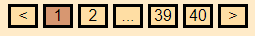
\includegraphics[scale=0.7]{images/application/pagination.png}
    \caption{Navigation és Subnavigation}
\end{figure}

A Pagination komponens más komponensekbe egyszerűen implementálható. Propsként meg kell kapnia a jelenlegi oldalt, valamint egy függvényt, ami az oldal változását kezeli. Azt, hogy a találatok közül hanyadik oldalnak kell betöltődnie, az implementáló komponensek tartják számon. Amikor a komponensek lekérik az elemeket az adatbázisból, akkor mellékelniük kell hogy hanyadik oldalt kérik, hogy hogy hány darab találatot kérnek.

\subsubsection{YearSelector komponens}
A YearSelector komponens lehetőséget biztosít, hogy egy lenyíló menüből a felhasználó évszámot választhasson.

\Section{A backend megvalósítása}
% TODO: Mivel a backend aránylag egyszerű szerkezetű, ezért itt elég csak röviden bemutatni, hogy a routing hogy lett megoldva, és hogy szerkezetileg hogy épül fel az alkalmazás.
A backend NodeJS és Express segítségével valósul meg. A NodeJS egy nyílt forráskódú JavaScript környezet, amelynek segítségével szerver alkalmazásokat lehet készíteni. Az Express egy minimális és rugalmas NodeJS keretrendszer.

\bigskip

A szerver alkalmazás az Express keretrendszeren kívül más modulokat is felhasznál:
\begin{itemize}
    \item A path modul: Fájl és mappa elérési útvonalakkal való dolgozáshoz ad eszközöket
    \item A morgan modul: Kérések naplózását végzi
    \item A cookie-parser és body-parser modulok: Kérések törzseit (?) és cookie-jainek elemzésére használatos
\end{itemize}

Az útvonalak a routes mappában találhatóak, és az index.js fájlban kerülnek importálásra. A config.js fájlban kerül inicializálásra a Neo4j driver.
